\documentclass{standalone}
\usepackage{tikz}
\usetikzlibrary{patterns, positioning}


\begin{document}
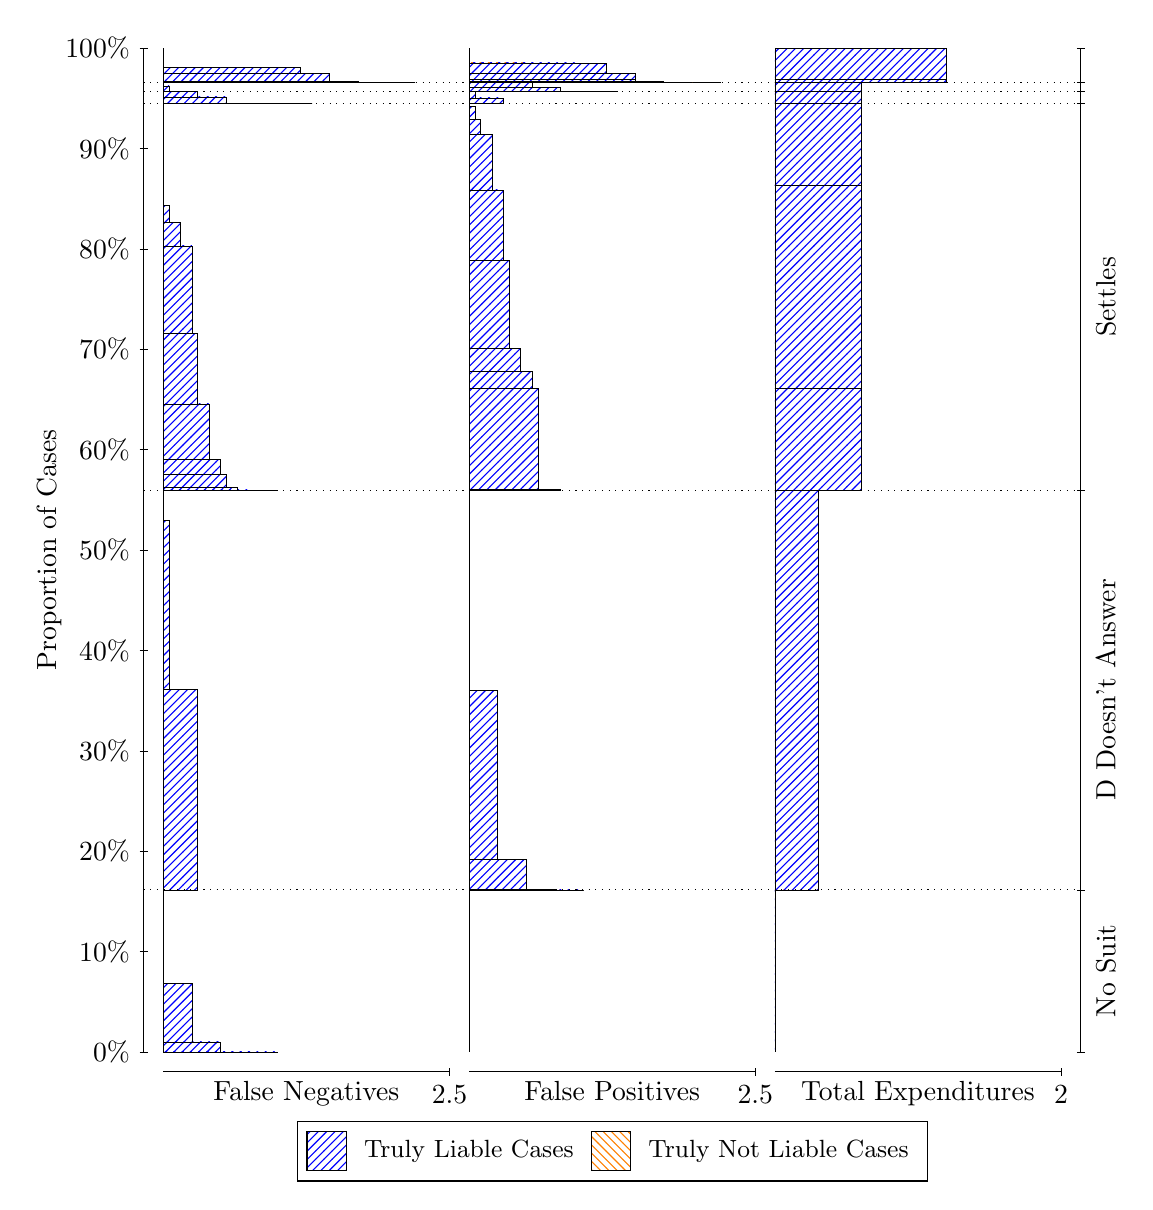
\begin{tikzpicture}
\draw[black, very thin] (1.5,1.75) -- (1.5,14.5);
\node[rotate=90, text=black, anchor=center] at (0.3, 8.125) {Proportion of Cases};
\draw[black, very thin] (1.45,1.75) -- (1.55,1.75);
\node[text=black, anchor=east] at (1.45, 1.75) {0\%};
\draw[black, very thin] (1.45,3.025) -- (1.55,3.025);
\node[text=black, anchor=east] at (1.45, 3.025) {10\%};
\draw[black, very thin] (1.45,4.3) -- (1.55,4.3);
\node[text=black, anchor=east] at (1.45, 4.3) {20\%};
\draw[black, very thin] (1.45,5.575) -- (1.55,5.575);
\node[text=black, anchor=east] at (1.45, 5.575) {30\%};
\draw[black, very thin] (1.45,6.85) -- (1.55,6.85);
\node[text=black, anchor=east] at (1.45, 6.85) {40\%};
\draw[black, very thin] (1.45,8.125) -- (1.55,8.125);
\node[text=black, anchor=east] at (1.45, 8.125) {50\%};
\draw[black, very thin] (1.45,9.4) -- (1.55,9.4);
\node[text=black, anchor=east] at (1.45, 9.4) {60\%};
\draw[black, very thin] (1.45,10.675) -- (1.55,10.675);
\node[text=black, anchor=east] at (1.45, 10.675) {70\%};
\draw[black, very thin] (1.45,11.95) -- (1.55,11.95);
\node[text=black, anchor=east] at (1.45, 11.95) {80\%};
\draw[black, very thin] (1.45,13.225) -- (1.55,13.225);
\node[text=black, anchor=east] at (1.45, 13.225) {90\%};
\draw[black, very thin] (1.45,14.5) -- (1.55,14.5);
\node[text=black, anchor=east] at (1.45, 14.5) {100\%};

\draw[black, very thin] (13.4,1.75) -- (13.4,14.5);
\draw[black, very thin] (13.35,1.75) -- (13.45,1.75);
\node[anchor=west] at (13.35, 1.75) {};
\draw[black, very thin] (13.35,3.8088) -- (13.45,3.8088);
\node[anchor=west] at (13.35, 3.8088) {};
\draw[black, very thin] (13.35,8.8854) -- (13.45,8.8854);
\node[anchor=west] at (13.35, 8.8854) {};
\draw[black, very thin] (13.35,13.793) -- (13.45,13.793);
\node[anchor=west] at (13.35, 13.793) {};
\draw[black, very thin] (13.35,13.953) -- (13.45,13.953);
\node[anchor=west] at (13.35, 13.953) {};
\draw[black, very thin] (13.35,14.066) -- (13.45,14.066);
\node[anchor=west] at (13.35, 14.066) {};
\draw[black, very thin] (13.35,14.5) -- (13.45,14.5);
\node[anchor=west] at (13.35, 14.5) {};

\draw[black, very thin, pattern color=blue, pattern=north east lines] (1.75,1.75) rectangle (3.2033,1.75);
\draw[black, very thin, pattern color=blue, pattern=north east lines] (1.75,1.75) rectangle (2.84,1.7511);
\draw[black, very thin, pattern color=blue, pattern=north east lines] (1.75,1.7511) rectangle (2.4767,1.8784);
\draw[black, very thin, pattern color=blue, pattern=north east lines] (1.75,1.8784) rectangle (2.1133,2.625);
\draw[black, very thin, pattern color=orange, pattern=north west lines] (1.75,2.625) rectangle (1.75,2.625);
\draw[black, very thin, pattern color=blue, pattern=north east lines] (1.75,2.625) rectangle (1.75,3.8088);
\draw[black, very thin, pattern color=blue, pattern=north east lines] (1.75,3.8088) rectangle (2.186,6.3546);
\draw[black, very thin, pattern color=blue, pattern=north east lines] (1.75,6.3546) rectangle (1.8227,8.4986);
\draw[black, very thin, pattern color=orange, pattern=north west lines] (1.75,8.4986) rectangle (1.75,8.4986);
\draw[black, very thin, pattern color=blue, pattern=north east lines] (1.75,8.4986) rectangle (1.75,8.8854);
\draw[black, very thin, pattern color=blue, pattern=north east lines] (1.75,8.8854) rectangle (3.2033,8.8854);
\draw[black, very thin, pattern color=blue, pattern=north east lines] (1.75,8.8854) rectangle (3.058,8.8854);
\draw[black, very thin, pattern color=blue, pattern=north east lines] (1.75,8.8854) rectangle (2.9127,8.8858);
\draw[black, very thin, pattern color=blue, pattern=north east lines] (1.75,8.8858) rectangle (2.84,8.8872);
\draw[black, very thin, pattern color=blue, pattern=north east lines] (1.75,8.8872) rectangle (2.6947,8.916);
\draw[black, very thin, pattern color=blue, pattern=north east lines] (1.75,8.916) rectangle (2.5493,9.0899);
\draw[black, very thin, pattern color=blue, pattern=north east lines] (1.75,9.0899) rectangle (2.4767,9.28);
\draw[black, very thin, pattern color=blue, pattern=north east lines] (1.75,9.28) rectangle (2.3313,9.9798);
\draw[black, very thin, pattern color=blue, pattern=north east lines] (1.75,9.9798) rectangle (2.186,10.878);
\draw[black, very thin, pattern color=blue, pattern=north east lines] (1.75,10.878) rectangle (2.1133,11.988);
\draw[black, very thin, pattern color=blue, pattern=north east lines] (1.75,11.988) rectangle (1.968,12.288);
\draw[black, very thin, pattern color=blue, pattern=north east lines] (1.75,12.288) rectangle (1.8227,12.502);
\draw[black, very thin, pattern color=orange, pattern=north west lines] (1.75,12.502) rectangle (1.75,12.502);
\draw[black, very thin, pattern color=blue, pattern=north east lines] (1.75,12.502) rectangle (1.75,13.793);
\draw[black, very thin, pattern color=blue, pattern=north east lines] (1.75,13.793) rectangle (3.6393,13.793);
\draw[black, very thin, pattern color=blue, pattern=north east lines] (1.75,13.793) rectangle (3.276,13.793);
\draw[black, very thin, pattern color=blue, pattern=north east lines] (1.75,13.793) rectangle (2.9127,13.795);
\draw[black, very thin, pattern color=blue, pattern=north east lines] (1.75,13.795) rectangle (2.5493,13.88);
\draw[black, very thin, pattern color=blue, pattern=north east lines] (1.75,13.88) rectangle (2.186,13.953);
\draw[black, very thin, pattern color=orange, pattern=north west lines] (1.75,13.953) rectangle (1.75,13.953);
\draw[black, very thin, pattern color=blue, pattern=north east lines] (1.75,13.953) rectangle (2.186,13.954);
\draw[black, very thin, pattern color=blue, pattern=north east lines] (1.75,13.954) rectangle (1.8227,14.019);
\draw[black, very thin, pattern color=orange, pattern=north west lines] (1.75,14.019) rectangle (1.75,14.019);
\draw[black, very thin, pattern color=blue, pattern=north east lines] (1.75,14.019) rectangle (1.75,14.066);
\draw[black, very thin, pattern color=blue, pattern=north east lines] (1.75,14.066) rectangle (4.9473,14.066);
\draw[black, very thin, pattern color=blue, pattern=north east lines] (1.75,14.066) rectangle (4.584,14.066);
\draw[black, very thin, pattern color=blue, pattern=north east lines] (1.75,14.066) rectangle (4.2207,14.074);
\draw[black, very thin, pattern color=blue, pattern=north east lines] (1.75,14.074) rectangle (3.8573,14.173);
\draw[black, very thin, pattern color=blue, pattern=north east lines] (1.75,14.173) rectangle (3.494,14.256);
\draw[black, very thin, pattern color=blue, pattern=north east lines] (1.75,14.256) rectangle (3.1307,14.256);
\draw[black, very thin, pattern color=blue, pattern=north east lines] (1.75,14.256) rectangle (2.84,14.256);
\draw[black, very thin, pattern color=blue, pattern=north east lines] (1.75,14.256) rectangle (2.7673,14.256);
\draw[black, very thin, pattern color=blue, pattern=north east lines] (1.75,14.256) rectangle (2.4767,14.256);
\draw[black, very thin, pattern color=blue, pattern=north east lines] (1.75,14.256) rectangle (2.1133,14.257);
\draw[black, very thin, pattern color=orange, pattern=north west lines] (1.75,14.257) rectangle (1.75,14.257);
\draw[black, very thin, pattern color=blue, pattern=north east lines] (1.75,14.257) rectangle (1.75,14.5);
\draw[black, very thin, pattern color=orange, pattern=north west lines] (5.6333,1.75) rectangle (5.6333,1.75);
\draw[black, very thin, pattern color=blue, pattern=north east lines] (5.6333,1.75) rectangle (5.6333,3.8088);
\draw[black, very thin, pattern color=orange, pattern=north west lines] (5.6333,3.8088) rectangle (7.0867,3.8088);
\draw[black, very thin, pattern color=blue, pattern=north east lines] (5.6333,3.8088) rectangle (7.0867,3.8088);
\draw[black, very thin, pattern color=blue, pattern=north east lines] (5.6333,3.8088) rectangle (6.7233,3.8112);
\draw[black, very thin, pattern color=blue, pattern=north east lines] (5.6333,3.8112) rectangle (6.36,4.1956);
\draw[black, very thin, pattern color=blue, pattern=north east lines] (5.6333,4.1956) rectangle (5.9967,6.3396);
\draw[black, very thin, pattern color=blue, pattern=north east lines] (5.6333,6.3396) rectangle (5.6333,8.8854);
\draw[black, very thin, pattern color=orange, pattern=north west lines] (5.6333,8.8854) rectangle (6.796,8.8854);
\draw[black, very thin, pattern color=blue, pattern=north east lines] (5.6333,8.8854) rectangle (6.796,8.8907);
\draw[black, very thin, pattern color=orange, pattern=north west lines] (5.6333,8.8907) rectangle (6.6507,8.8907);
\draw[black, very thin, pattern color=blue, pattern=north east lines] (5.6333,8.8907) rectangle (6.6507,8.8988);
\draw[black, very thin, pattern color=orange, pattern=north west lines] (5.6333,8.8988) rectangle (6.5053,8.8988);
\draw[black, very thin, pattern color=blue, pattern=north east lines] (5.6333,8.8988) rectangle (6.5053,10.176);
\draw[black, very thin, pattern color=blue, pattern=north east lines] (5.6333,10.176) rectangle (6.4327,10.39);
\draw[black, very thin, pattern color=blue, pattern=north east lines] (5.6333,10.39) rectangle (6.2873,10.69);
\draw[black, very thin, pattern color=blue, pattern=north east lines] (5.6333,10.69) rectangle (6.142,11.801);
\draw[black, very thin, pattern color=blue, pattern=north east lines] (5.6333,11.801) rectangle (6.0693,12.699);
\draw[black, very thin, pattern color=blue, pattern=north east lines] (5.6333,12.699) rectangle (5.924,13.399);
\draw[black, very thin, pattern color=blue, pattern=north east lines] (5.6333,13.399) rectangle (5.7787,13.589);
\draw[black, very thin, pattern color=blue, pattern=north east lines] (5.6333,13.589) rectangle (5.706,13.763);
\draw[black, very thin, pattern color=blue, pattern=north east lines] (5.6333,13.763) rectangle (5.6333,13.793);
\draw[black, very thin, pattern color=orange, pattern=north west lines] (5.6333,13.793) rectangle (6.0693,13.793);
\draw[black, very thin, pattern color=blue, pattern=north east lines] (5.6333,13.793) rectangle (6.0693,13.867);
\draw[black, very thin, pattern color=blue, pattern=north east lines] (5.6333,13.867) rectangle (5.706,13.951);
\draw[black, very thin, pattern color=blue, pattern=north east lines] (5.6333,13.951) rectangle (5.6333,13.953);
\draw[black, very thin, pattern color=orange, pattern=north west lines] (5.6333,13.953) rectangle (7.5227,13.953);
\draw[black, very thin, pattern color=blue, pattern=north east lines] (5.6333,13.953) rectangle (7.5227,13.953);
\draw[black, very thin, pattern color=blue, pattern=north east lines] (5.6333,13.953) rectangle (7.1593,13.953);
\draw[black, very thin, pattern color=blue, pattern=north east lines] (5.6333,13.953) rectangle (6.796,14);
\draw[black, very thin, pattern color=blue, pattern=north east lines] (5.6333,14) rectangle (6.4327,14.065);
\draw[black, very thin, pattern color=blue, pattern=north east lines] (5.6333,14.065) rectangle (6.0693,14.066);
\draw[black, very thin, pattern color=orange, pattern=north west lines] (5.6333,14.066) rectangle (8.8307,14.066);
\draw[black, very thin, pattern color=blue, pattern=north east lines] (5.6333,14.066) rectangle (8.8307,14.066);
\draw[black, very thin, pattern color=blue, pattern=north east lines] (5.6333,14.066) rectangle (8.4673,14.066);
\draw[black, very thin, pattern color=orange, pattern=north west lines] (5.6333,14.066) rectangle (8.4673,14.066);
\draw[black, very thin, pattern color=blue, pattern=north east lines] (5.6333,14.066) rectangle (8.4673,14.066);
\draw[black, very thin, pattern color=blue, pattern=north east lines] (5.6333,14.066) rectangle (8.104,14.071);
\draw[black, very thin, pattern color=orange, pattern=north west lines] (5.6333,14.071) rectangle (8.104,14.071);
\draw[black, very thin, pattern color=blue, pattern=north east lines] (5.6333,14.071) rectangle (8.104,14.073);
\draw[black, very thin, pattern color=blue, pattern=north east lines] (5.6333,14.073) rectangle (7.7407,14.105);
\draw[black, very thin, pattern color=orange, pattern=north west lines] (5.6333,14.105) rectangle (7.7407,14.105);
\draw[black, very thin, pattern color=blue, pattern=north east lines] (5.6333,14.105) rectangle (7.7407,14.173);
\draw[black, very thin, pattern color=blue, pattern=north east lines] (5.6333,14.173) rectangle (7.3773,14.175);
\draw[black, very thin, pattern color=blue, pattern=north east lines] (5.6333,14.175) rectangle (7.3773,14.309);
\draw[black, very thin, pattern color=blue, pattern=north east lines] (5.6333,14.309) rectangle (7.014,14.31);
\draw[black, very thin, pattern color=blue, pattern=north east lines] (5.6333,14.31) rectangle (6.6507,14.31);
\draw[black, very thin, pattern color=orange, pattern=north west lines] (5.6333,14.31) rectangle (6.36,14.31);
\draw[black, very thin, pattern color=blue, pattern=north east lines] (5.6333,14.31) rectangle (6.36,14.31);
\draw[black, very thin, pattern color=blue, pattern=north east lines] (5.6333,14.31) rectangle (6.2873,14.31);
\draw[black, very thin, pattern color=orange, pattern=north west lines] (5.6333,14.31) rectangle (5.9967,14.31);
\draw[black, very thin, pattern color=blue, pattern=north east lines] (5.6333,14.31) rectangle (5.9967,14.311);
\draw[black, very thin, pattern color=orange, pattern=north west lines] (5.6333,14.311) rectangle (5.6333,14.311);
\draw[black, very thin, pattern color=blue, pattern=north east lines] (5.6333,14.311) rectangle (5.6333,14.5);
\draw[black, very thin, pattern color=orange, pattern=north west lines] (9.5167,1.75) rectangle (9.5167,1.75);
\draw[black, very thin, pattern color=blue, pattern=north east lines] (9.5167,1.75) rectangle (9.5167,3.8088);
\draw[black, very thin, pattern color=orange, pattern=north west lines] (9.5167,3.8088) rectangle (10.062,3.8088);
\draw[black, very thin, pattern color=blue, pattern=north east lines] (9.5167,3.8088) rectangle (10.062,8.8854);
\draw[black, very thin, pattern color=orange, pattern=north west lines] (9.5167,8.8854) rectangle (10.607,8.8854);
\draw[black, very thin, pattern color=blue, pattern=north east lines] (9.5167,8.8854) rectangle (10.607,10.177);
\draw[black, very thin, pattern color=orange, pattern=north west lines] (9.5167,10.177) rectangle (10.607,10.177);
\draw[black, very thin, pattern color=blue, pattern=north east lines] (9.5167,10.177) rectangle (10.607,12.756);
\draw[black, very thin, pattern color=orange, pattern=north west lines] (9.5167,12.756) rectangle (10.607,12.756);
\draw[black, very thin, pattern color=blue, pattern=north east lines] (9.5167,12.756) rectangle (10.607,13.793);
\draw[black, very thin, pattern color=orange, pattern=north west lines] (9.5167,13.793) rectangle (10.607,13.793);
\draw[black, very thin, pattern color=blue, pattern=north east lines] (9.5167,13.793) rectangle (10.607,13.953);
\draw[black, very thin, pattern color=orange, pattern=north west lines] (9.5167,13.953) rectangle (10.607,13.953);
\draw[black, very thin, pattern color=blue, pattern=north east lines] (9.5167,13.953) rectangle (10.607,14.066);
\draw[black, very thin, pattern color=orange, pattern=north west lines] (9.5167,14.066) rectangle (11.697,14.066);
\draw[black, very thin, pattern color=blue, pattern=north east lines] (9.5167,14.066) rectangle (11.697,14.104);
\draw[black, very thin, pattern color=orange, pattern=north west lines] (9.5167,14.104) rectangle (11.697,14.104);
\draw[black, very thin, pattern color=blue, pattern=north east lines] (9.5167,14.104) rectangle (11.697,14.5);
\draw[black, dotted] (1.5,3.8088) -- (13.4,3.8088);
\draw[black, dotted] (1.5,8.8854) -- (13.4,8.8854);
\draw[black, dotted] (1.5,13.793) -- (13.4,13.793);
\draw[black, dotted] (1.5,13.953) -- (13.4,13.953);
\draw[black, dotted] (1.5,14.066) -- (13.4,14.066);
\draw[black, very thin] (1.75,1.5) -- (5.3833,1.5);
\node[text=black, anchor=north] at (3.5667, 1.5) {False Negatives};
\draw[black, very thin] (5.3833,1.45) -- (5.3833,1.55);
\node[text=black, anchor=north] at (5.3833, 1.45) {2.5};

\draw[black, very thin] (5.6333,1.5) -- (9.2667,1.5);
\node[text=black, anchor=north] at (7.45, 1.5) {False Positives};
\draw[black, very thin] (9.2667,1.45) -- (9.2667,1.55);
\node[text=black, anchor=north] at (9.2667, 1.45) {2.5};

\draw[black, very thin] (9.5167,1.5) -- (13.15,1.5);
\node[text=black, anchor=north] at (11.333, 1.5) {Total Expenditures};
\draw[black, very thin] (13.15,1.45) -- (13.15,1.55);
\node[text=black, anchor=north] at (13.15, 1.45) {2};

\node[text=black, centered, rotate=90] at (13.72, 2.7794) {No Suit};
\node[text=black, centered, rotate=90] at (13.72, 6.3471) {D Doesn't Answer};
\node[text=black, centered, rotate=90] at (13.72, 11.339) {Settles};




\draw (7.449999999999999,1.5) node[draw=none] (baseCoordinate) {};
\begin{scope}[align=center]
        \matrix[scale=0.5, draw=black, below=0.5cm of baseCoordinate, nodes={draw}, column sep=0.1cm]{
            \node[rectangle, draw, minimum width=0.5cm, minimum height=0.5cm, pattern color=blue, pattern=north east lines] {}; &
            \node[draw=none, font=\small, text=black] (B) {Truly Liable Cases}; &
            \node[rectangle, draw, minimum width=0.5cm, minimum height=0.5cm, pattern color=orange, pattern=north west lines] {}; &
            \node[draw=none, font=\small, text=black] (B) {Truly Not Liable Cases}; \\
            };
\end{scope}

\end{tikzpicture}
\end{document}